\documentclass{article}

\usepackage{graphicx} % Used for images

\usepackage{listings} %For code
\lstset{ % Code block styling
  basicstyle=\ttfamily,
  columns=fullflexible,
  frame=lines,
  breaklines=true,
}

% Setup table of contents links
\usepackage{color}   %May be necessary if you want to color links
\usepackage{hyperref}
\hypersetup{
    colorlinks=true, %set true if you want colored links
    linktoc=all,     %set to all if you want both sections and subsections linked
    linkcolor=blue,  %choose some color if you want links to stand out
}

\title{%
	Project 1 Project Page\\
    \large CISC 191-86930}
\author{Alexandra Steiner}

\begin{document}
\maketitle

\tableofcontents

\newpage

\section{Project Pitch}
For this project, I plan to create a command line utility that evaluates equations provided as text, and modifies then outputs the provided text to reflect the evaluation. This command line utility will be called from the command line as follows.

\begin{lstlisting} 
evaluate [options...] [-w -write [filepath]]
	[-f -file [filepath]] | [-t -text [textinput]] 
\end{lstlisting}

\subsection{Options:}
\begin{itemize}
	\item \textbf{-w -write {[\textless filepath\textgreater]}} Writes the evaluated output to a file at the specified path. If a file at the path already exists, overwrites the file. If no file exists, tries to create a file. If this option is selected, the results of the evaluation will not be written to the output stream
	\item \textbf{-f -file {[\textless filepath\textgreater]}} Attempts to read text from the provided file path and evaluate it as an equation \footnote{If executed with the \textbf{-t -text} option, will evaluate provided text as seperate equation(s)}
	\item \textbf{-t -text {[\textless textinput\textgreater]}} Attempts to evaluate the provided text input as an equation \footnote{If executed with the \textbf{-f -file} option, will evaluate provided text as seperate equation(s)}
	\item \textbf{-h -help} Displays the help message
	\item \textbf{-v -version} Displays version and program information
	\item \textbf{-q -quiet} Does not write the results of the evaluation to the output stream. Results are written to the output stream by default
\end{itemize}

\subsection{Scope of Evaluation}
Since coding in every operator and mathematical quirk would be beyond the scope of this project, only the below specified operators are valid. Additionally, dealing with variables is beyond the scope of this project, so all values separated by operators must be numeric.
\subsubsection{Valid Operators}
\begin{itemize}
	\item \fbox{\textbf{x+y}} Adds x and y (Add, Binary)
	\item \fbox{\textbf{x-y}} Subtracts y from x (Subtract, Binary)
	\item \fbox{\textbf{x*y}} Multiplies x by y (Multiply, Binary)
	\item \fbox{\textbf{x/y}} Divides x by y (Divide, Binary)
	\item \fbox{\textbf{-x}} Negates x (Prefix Operator Only) (Negate, Unary)
	\item \fbox{\textbf{x=y}} Checks x and y for equality (Equate, Binary)
\end{itemize}

\subsection{Equation Processing}
Equations are always provided to the evaluate utility as a text. Before processing, the provided text is checked for illegal characters and illegal syntax. Provided text may contain multiple equation separated by new lines.

Equation may be provided to the evaluate utility as a file path, a command argument, or through Java's InputStream as detailed in the command line option specifications. Equations may be provided in the following formats. Assume "expression" is a valid expression and "evaluation" is the evaluation of expression.

\begin{itemize}
	\item "expression" is processed into "expression = evaluation"
	\item "expression = " is processed into "expression = evaluation"
	\item "expression = expression" is processed into "expression = expression is true/false/unsolvable"
\end{itemize}

An equation is considered valid when:
\begin{enumerate}
	\item The text of the equation only contains valid characters. Valid characters are all numeric characters, the period, and all valid operators (+-*/=). Expressions may not contain new lines
	\item The equation is provided in a valid format (detailed above)
	\item The equation's syntax is valid
\end{enumerate}

\subsection{Program Examples}
\begin{lstlisting}[title=myEquation.txt]
(1+2+3)/4
10*15-4 = 15
\end{lstlisting}

\begin{lstlisting}[title=Commands]
evaluate -v
>> evaluate version 2.45
>> Created by author for CISC 191

evaluate -t "1+2+4/2"
>> 1+2+4/2 = 5

evaluate -t "18 = 36/2"
>> 18 = 36/2 is true

evaluate -t "18 = "
>> 18 = 18

evaluate << myEquation.txt
>> (1+2+3)/4 = 1.5
>> 10*15-4 = 15 is false

evaluate -f myEquation.txt
>> (1+2+3)/4 = 1.5
>> 10*15-4 = 15 is false

evaluate -f myEquation.txt -w myEquation.txt
\end{lstlisting}

\begin{lstlisting}[title=myEquation.txt after commands are executed]
(1+2+3)/4 = 1.5
10*15-4 = 15 is false
\end{lstlisting}

\section{UML Diagram}
See figure \ref{fig:Project 1 UML Diagram} for this project's uml diagram.

\begin{figure}[h]
  	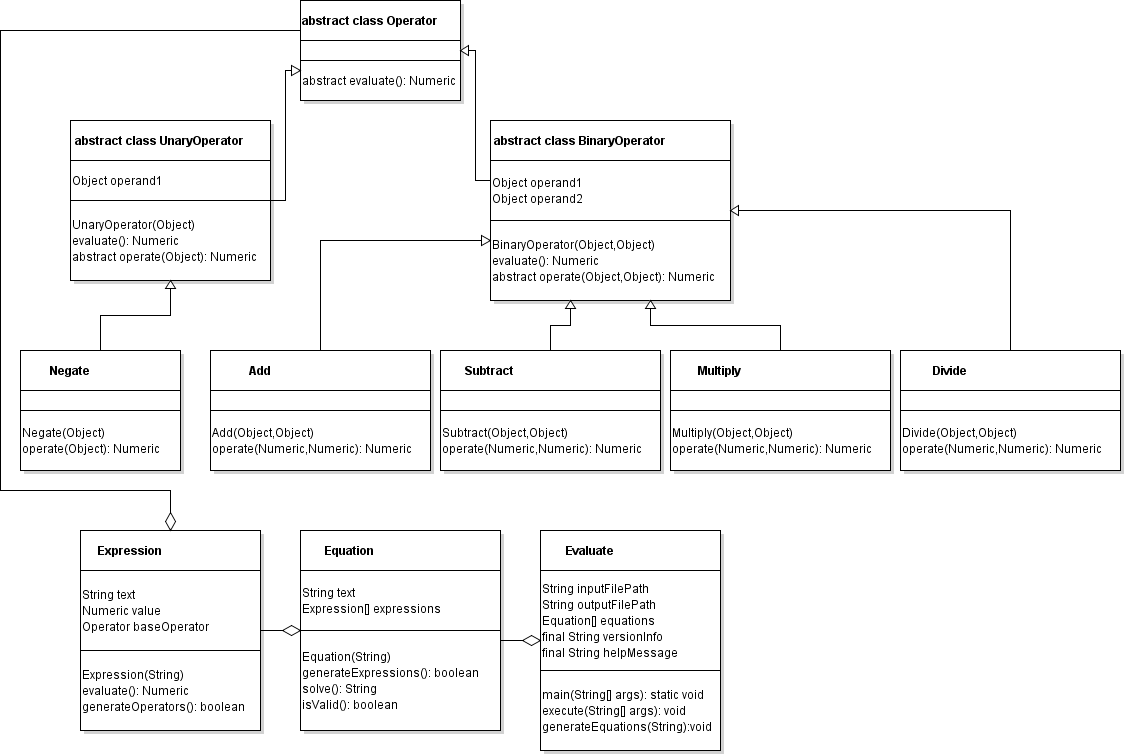
\includegraphics[width=1\textwidth]{Project1UML_1.png}
  	\caption{The UML Diagram for the evaluate utility}
  	\label{fig:Project 1 UML Diagram}
\end{figure}

\section{Learning Outcomes}
\subsection{LO1: Employ design principles of object-oriented programming}
This program will use the divide and conquer principle of OOP to divide equations into smaller pieces that will interact with each other. While equations can be solved without OOP, dividing equations into many smaller pieces allows for more flexibility and the easy addition of additional operators down the road
\subsection{LO2: Construct programs utilizing single and multidimensional arrays}
This project will use arrays to store equations and equation components. Multi-dimensional arrays will be used to preform a syntax check on equations before processing to improve efficiency.
\subsection{LO3: Construct programs utilizing object and classes in object-oriented programming, including aggregation}
This program will store equations as classes, aggregating a number of different numeric and operator classes that represent the equation. The equation class will also contain a String, which is another example of class aggregation.
\subsection{LO4: Construct programs utilizing inheritance and polymorphism, including abstract classes and interfaces}
This program uses inheritance to eliminate redundant code when create operators. Additionally, operator operands use polymorphism to store either Numeric values or Operator values. This gives operators more flexibility. Moreover, numeric values benefit from polymorphism since some values are better stored as integer values and other values are better stored as decimal values.
\subsection{LO5: Construct programs utilizing exception handling}
Since this program will attempt to read and write to file paths, utilizing exception handling is a must to ensure that users trying to read equations from thisfiledoesnotexist.docx will not get an ugly face-full of Java error.
\subsection{LO6: Construct programs utilizing text file I/O}
File IO will be used to handle file input / output as specified in the project pitch

\section{Work Schedule}
I will be working on this project at approximately 1-4 pm on Saturdays and likely sporadically throughout the week whenever I can make time.
\section{Timeline}
\subsection{Week 1}
\begin{itemize}
	\item Write the project proposal
	\item Plan the code. Determine classes (with fields and methods) and interfaces and their responsibilities
	\item Create project page
\end{itemize}
\subsection{Week 2}
\begin{itemize}
	\item Create framework for all classes (define methods, fields, and classes as specified in figure \ref{fig:Project 1 UML Diagram}).
	\item Flesh out Evaluate class so project has a working user interface going forwards
	\item Develop test cases and create JUnit tests
	\item Determine where exception handling is needed to ensure the program fails gracefully
	\item Update project page with progress details
	\item Submit code written so far
\end{itemize}
\subsection{Week 3}
\begin{itemize}
	\item Finish writing classes
	\item Test and debug code
	\item Work out any edge cases and add to JUnit tests
	\item Update project page with progress details
	\item Submit code written so far
\end{itemize}
\subsection{Week 4}
\begin{itemize}
	\item Debug any remaining problems
	\item Create project demonstration supporting files and figures
	\item Create project demonstration video, including information about how each LO is used as part of the project
	\item Submit final code on Canvas and add videos to project page
\end{itemize}

\end{document}